\documentclass[12pt]{article}
    \usepackage[utf8]{inputenc}
    \usepackage{hyperref}
    \usepackage{graphicx}
    \usepackage{fancyhdr}
    \usepackage{geometry}  % Adjusting document margins

    % Adjust document margins
    \geometry{left=1in, right=1in, top=1in, bottom=1in}

    \pagestyle{fancy}
    \fancyhf{} % Clear all header and footer fields
    \renewcommand{\headrulewidth}{0pt} % No line in header
    \renewcommand{\footrulewidth}{0pt} % No line in footer

    % Custom title with bold and larger font
    \title{\vspace{-2cm} % Adjust the vertical space as needed
           \Huge\textbf{Clima Craft Report} \\ [0.5cm]  % Making the title big and bold
           \Large{your lightweight LaTeX weather report} % Subtitle in a slightly smaller size
           \vspace{0.5cm} \\ \hrule \vspace{-0.2cm} \hrule
    }
    \author{}
    \date{}

    \begin{document}
    \maketitle
    \fancyhead[L]{\textbf{\large Clima Craft Report}}  % Left header: Custom title, bold and larger
    \section*{Weather at a Glance }
At a cool 6.0°C, the air whispers of change, brisk and refreshing. It hints at the need for a warm layer, inviting a sense of calm and a breath of fresh air. This gentle reminder of the season's shift encourages one to savor the crispness that envelops the surroundings. Above, the skies of Freiburg don a cloak of partly cloudy, setting the stage for the day's mood. A wind, carrying whispers at 3.6 kph from the S, shapes the air's embrace. The atmosphere, pressing down with a pressure of 1017.0 mb, remains unseen but deeply felt, a silent guardian of the day. Humidity at 81% weaves a tale of invisible waters binding earth and sky, while clouds, those fleeting masterpieces, adorn 75% of the heavens. This dance of light and shadow plays over the landscape, with the mercury hinting at 6.0°C yet the sensation on the skin echoes 5.0°C. Visibility stretches to 10.0 km, promising clear views that invite the soul to wander. Together, these elements weave a tapestry of weather in Freiburg, not merely a story of data but an experience woven from the sun's warmth, the wind's caress, and the clouds' silent passage. Here, in the heart of Freiburg, the day unfolds with a promise of moments lived under an ever-changing sky, a narrative rich with the essence of life itself.
\paragraph{}This graph provides a clear idea about the temperature and precipitation in Freiburg.
\begin{figure}[h]
\centering
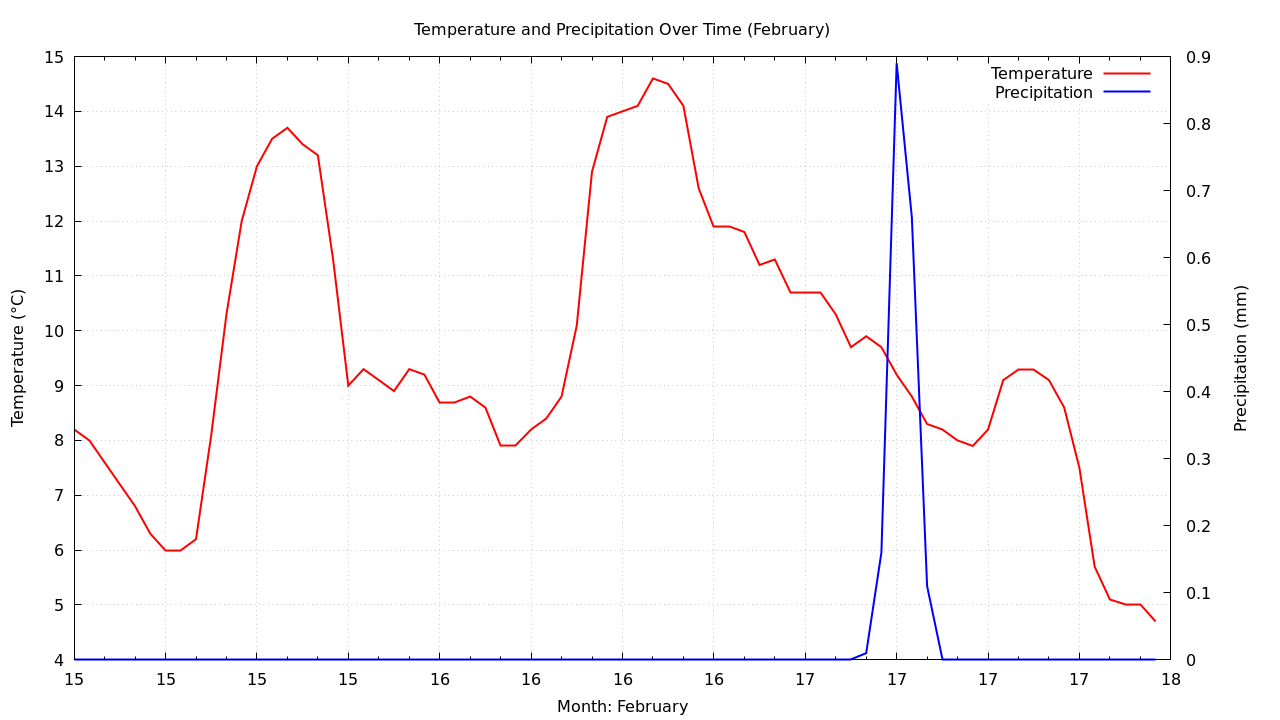
\includegraphics[width=0.8\textwidth]{data/graph/temperature_precipitation_graph.png}
\caption{Temperature and Precipitation Overview in Freiburg}
\end{figure}

\end{document}